\documentclass[12pt]{article}
\usepackage[a4paper]{}
\usepackage{graphicx}
\usepackage[utf8]{inputenc}
\usepackage{amsmath}
\usepackage[]{algorithm2e}
\usepackage{comment}
\usepackage{soul}
\usepackage{cancel}
\usepackage{multirow}
\usepackage{chngcntr}
\usepackage{enumitem}
\usepackage{booktabs}
\usepackage[table,xcdraw]{xcolor}
\counterwithin{table}{section}
\usepackage{subfigure}
\usepackage{array}
\usepackage{float}
\restylefloat{table}
\graphicspath{ {images/} }
%\topmargin 15mm
\numberwithin{figure}{section}
\providecommand{\keywords}[1]{\textbf{\textit{Keywords---}} #1}
\headheight 10pt
\oddsidemargin 0mm
%\evensidemargin -5mm
\textwidth 161mm
\textheight 210mm
\linespread{1.3}
\begin{document}
\thispagestyle{empty}
 \begin{center}
Major Project Proposal Report\\
\null
on\\
\null
\textbf{Automatic Generation of Medical Imaging Reports}\\
\null
Submitted by \\
\null
\textbf{Rahul Kumar}\\
\textbf{172IT014}\\
\textbf{M.Tech (IT)}\\
\null
Under the Guidance of\\
\textbf{Dr. Sownmya Kamath S.}  \\
\null
\textbf{Dept. of Information Technology,}\\
\textbf{NITK, Surathkal}\\
\null
\textbf{Date of Submission: 18-10-2018}\\
\begin{figure}[h] % b - bottom, t - top, h - here
 \centering{
 
\includegraphics[scale=0.7]{logo.jpg}
 }
\end{figure}
\textbf{Department of Information Technology\\
National Institute of Technology Karnataka, Surathkal\\
2018-2019}\\
\end{center}
\clearpage
\thispagestyle{empty}
\begin{center}
\underline{\textbf{CERTIFICATE}} \\
\end{center}
\null
This is to certify that the major project entitled "Automatic Generation of Medical Imaging Reports" is a bonafide work carried out as part of the course Major Project (IT898), under my guidance by Rahul Kumar, student of III Semester M.Tech (IT) at the Department of Information Technology, National Institute of Technology Karnataka, Surathkal, during the academic semester Jul - Nov 2018, in partial fulfillment of the requirements for the award of the degree of Master of Technology in Information Technology, at NITK Surathkal. 
\\
\\
\\
\\
\\
\\
\begin{minipage}{0.4\textwidth}
\begin{flushleft}
Signature of the Student\\
Place: Mangalore\\ 
Date:28-09-2018\\
\end{flushleft}
\end{minipage}
\begin{minipage}{0.4\textwidth}
\begin{flushright}
Signature of the Instructor(s)\\
\end{flushright}
\end{minipage}
\\
\\
\\
\clearpage
\thispagestyle{empty}
\begin{center}
\underline{\textbf{DECLARATION}}\\
\end{center}
\null
I hereby declare that the Major Project entitled “Automatic Generation of Medical Imaging Reports” submitted as part of the partial course requirements for the course Major Project (IT898) , for the award of the degree of Master of Technology in Information Technology at NITK Surathkal during the Jul - Nov 2018 semester, has been carried out by me. I declare that the project has not formed the basis for the award of any degree, associate ship, fellowship or any other similar titles elsewhere.\\ 
\\
\\
\\
\\
\\
\\
Signature of the Student\\
Place: Mangalore\\
Date:28-09-2018\\
\clearpage
\pagenumbering{roman}
\section*{Abstract}
Apart from being an interesting computer-vision problem, manual analysis of radiology images also needs to be performed by experienced radiologist which makes this issue even more necessary to be addressed. Automatic description generation for radiology images can benefit radiologist with quick, localised and explanatory analysis. Expected analysis must contain keywords (Tags) that images relates with, observation for different body parts in the image ( Findings), and the diagnosis ( Impression ).
Our goal here is comprises of three tasks, to classify given X-ray image against list of medical abnormalities resulting in tagged images, to generate narration along with localising region for found abnormalities, and finally using hierarchical LSTM, generating long report description .
We are 

\\
Keywords - Machine learning, GAN, deep learning, neural nets, DCGAN.
\\
\clearpage
\tableofcontents
\clearpage
\listoffigures 
\listoftables
\clearpage
\pagenumbering{arabic}
\section{Introduction}
\paragraph{}
Medical images
Radiologist analyse and diagnose using medical images for various diseases on a daily basis. However analysis, reading and interpretation, and writing textual report demands skills such as knowledge of anatomy and basic details about the visual symptoms of the disease, knowledge of correlation with other diagnostic results like pathology result etc.
Writing diagnostic report for radiology image, even for experienced radiologists is a time consuming process. And this same task sometimes is required to be repeated for up to hundreds of different radiology images everyday.
\paragraph{}
Medical reporting task and parts of report
Medical reporting procedure for radiology images include radiologist analysing various part of patient’s body and remarking various findings about those body parts. Sometimes different related or unrelated findings about different body parts can be observed in single images. Those findings and other observation then lead to a further consolidated overall diagnostic report about the patient known as Impression. In this process images needs to be given proper tags for future categorization and quick analysis purpose.
\paragraph{}
So our challenge is to provide solution for generating tags, findings and impression for a given radiology image. As the process of diagnostic, our challenge is can be broken down in three stages, starting with tags generation for a given image. We are solving this problem by classifying the images against various pre-known labels and thus solving it as a multi-label classification problem. Tags generated at this step are preserved for future query purpose as well as as input for further processing of images. 
\paragraph{}
We will be using Generative adversarial networks for multi-label classification. For our task, we setup a GAN for generating new sample data and then classifying it for N+1 classes, representing N real classes for N labels and one class for fake data.
Various regions of an image may contain different information for different body parts, which can be related sometimes or to be looked as unrelated multiple diagnostic many other times. This task includes localising the image regions and then generating narration for those regions. We are using a co-attention mechanism for analysing given images and the tags generated in multi-label classification process for the given image simultaneously and provide semantic information which can be used for further processing along with previously generated tags information.
\paragraph{Co-attention:}
Generating paragraph of description using hierarchical LSTM
Our third task is to generate descriptions for imaging report summarizing the findings for various regions of images. Description are usually long paragraphs having multiple lines. So this task presents challenges as generating long paragraphs is a nontrivial task. We will be using hierarchical LSTM\cite{1} with co-attention mechanism for generating findings for various regions and then combining them and further processing for description summary generation.
\paragraph{}
To summarize, our multi-task learning framework  will be generating tags, sentences for findings and multi-sentence textual description for given radiology images.


\clearpage


\section{Literature Survey}
\subsection{Background Study}
\paragraph{}
It is very important to predict protein structures from protein sequences in molecular design and biological medicine design due to the close association between the protein structure and its function. A two-stage neural network has been used to predict protein secondary structure based on the position specific scoring matrices generated by PSI-BLAST \cite{3}. Using a new testing set based on a set of 187 unique folds, and three-way cross-validation based on structural similarity criteria rather than sequence similarity criteria used previously the method presented here (PSIPRED) achieved an average Q3 score of between 76.5\% to 78.3\% depending on the precise definition of observed secondary structure used.
\paragraph{}
A protein secondary structure prediction framework based on the Extreme learning machine was proposed by Guoren Wang, Yi Zhao and Di Wang in 2008 \cite{4}. They proposed an extreme learning machine (ELM) based protein secondary structure prediction framework which can provide good performance at extremely fast speed. They divided the proposed method in three steps: (i) the three secondary structures were independently predicted by a binary ELM classifier first; (ii) a probability based combination (PBC) method is then proposed to combine these binary prediction results into the expected three-classification results and (iii) a helix postprocessing (HPP) method is finally proposed to further improve the overall performance of the framework based on biological features.
\paragraph{}
Among many other approaches, genetic algorithm is found to be a promising cooperative computational method to solve protein structure prediction in a reasonable time \cite{5}. To automate the right choice of parameter values the influence of self-organization is adopted to design a new genetic operator to optimize the process of prediction. Torsion angles, the local structural parameters which define the backbone of protein are considered to encode the chromosome that enhances the quality of the confirmation. Newly designed self-configured genetic operators are used to develop self-organizing genetic algorithm to facilitate the accurate structure prediction.
\paragraph{}
Ab initio protein secondary structure (SS) predictions are utilized to generate tertiary structure predictions, which are increasingly demanded due to the rapid discovery of proteins \cite{6}. They developed an SS predictor that makes use of the position-specific scoring matrix generated by PSI-BLAST and deep learning network architectures, which they called DNSS. This deep learning network approach was used to predict SS for a fully independent test dataset of 198 proteins, achieving a Q3 accuracy of 80.7 percent and a Sov accuracy of 74.2 percent.
\paragraph{}
Protein secondary structure prediction improved by recurrent neural networks integrated with 2-dimensional convolutional neural networks \cite{7}. To integrate the information on both dimensions of the matrix, the amino-acid residue (time-step) dimension and the feature vector dimension, they proposed a hybrid deep learning framework, 2-dimensional convolutional bidirectional recurrent neural networks (2C-BRNNs), for improving the accuracy of 8-class secondary structure prediction. The proposed hybrid framework is to extract the discriminative local interactions between amino-acid residues by 2-dimensional convolutional neural networks (2DCNN), and then further captures long-range interactions between amino-acid residues by bidirectional gated recurrent units (BGRUs) or bidirectional long short-term memory (BLSTM).
\clearpage
\subsection{Outcome of Literature Survey}

\begin{table}[H]
\caption{Outcome of Literature Survey}
\label{Outcome of Literature Survey}
\centering
\resizebox{\textwidth}{!}{%
\begin{tabular}{|c|c|c|c|}
\hline
\rowcolor[HTML]{C0C0C0} 
\textbf{Authors} & \textbf{Method} & \textbf{Advantages} & \textbf{Limitations} \\ \hline
David T. Jones & \begin{tabular}[c]{@{}c@{}}Proteins Secondary\\ Structure Prediction\\ Based on Position\\ Specific Scoring\\ Matrix\end{tabular} & \begin{tabular}[c]{@{}c@{}}Using a new testing set\\ based on a set of 187\\ unique folds, and three\\ way cross-validation\\ based on structural\\ similarity.\end{tabular} & \begin{tabular}[c]{@{}c@{}}Takes too much time\\ for training the module\\ and predicting the\\ protein secondary
\\structure.\end{tabular} \\ \hline
\begin{tabular}[c]{@{}c@{}}Guoren Wang\\ et al.\end{tabular} & \begin{tabular}[c]{@{}c@{}}A protein secondary\\ structure prediction\\ framework based on\\ the Extreme\\ Learning Machine\end{tabular} & \begin{tabular}[c]{@{}c@{}}ELM is a new learning\\ method used in the training\\ of PSS framework which\\ consumes little training\\ time while achieving\\ high accuracy.\end{tabular} & \begin{tabular}[c]{@{}c@{}}Not much improvement\\ in the Q3 accuracy and\\ Segment Overlap (Sov)\\ score.\end{tabular} \\ \hline
\begin{tabular}[c]{@{}c@{}}Amouda\\ Venkatesan et al.\end{tabular} & \begin{tabular}[c]{@{}c@{}}Computational Approach\\ for Protein Structure\\ Prediction\end{tabular} & \begin{tabular}[c]{@{}c@{}}Contributes to the\\ prediction of a native-\\like structure by eliminating\\ the time constraint and\\ effort demand. Energy\\ of the predicted structure\\ is minimized to great\\ extent, which proves the\\ stability of protein. \end{tabular} & \begin{tabular}[c]{@{}c@{}}Tested only on two\\ peptides. Not focused on\\ the Q3 or Q8 accuracy\\ as well as not focused\\ on Sov accuracy.\end{tabular} \\ \hline
\begin{tabular}[c]{@{}c@{}}Matt Spencer\\ et al.\end{tabular} & \begin{tabular}[c]{@{}c@{}}A deep learning network\\ approach to ab initio\\ protein secondary\\ structure prediction\end{tabular} & \begin{tabular}[c]{@{}c@{}}Used multilayer deep\\ learning network with PSSM\\ and Atchley's factor.\\ Utilized a hybrid scoring\\ method that takes Q3\\ and Sov score into account\\ in an attempt to increase\\ the PSP accuracy.\end{tabular} & \begin{tabular}[c]{@{}c@{}}Not able to increase\\ the Q3 score\\ significantly.\end{tabular} \\ \hline
\end{tabular}
}
\end{table}
\paragraph{}
There are a significant amount of work already done in this field. But the problem of very high time consumption during the training of deep learning network \cite{3} or the problem of stagnating of the accuracy around 80 \% is still there \cite{6}. Extreme Learning Machine is able to reduce the training time significantly, but it did not able to improve the Q3 accuracy \cite{4}. In our work, we are using ELM to reduce the training time of our deep learning network framework and LSTM to help it to increase the Q3 accuracy.
 \subsection{Problem Statement}
 \paragraph{}
 To design and implement a deep learning network framework to predict the protein secondary structure from protein sequences using PSI-BLAST.
\subsection{Objectives}
\begin{itemize}
\item Set up PSI-BLAST and get position-specific scoring matrix.
\item Generation of Sequence profiles.
\item Training of deep learning network architectures.
\item Prediction of protein secondary structure and post processing of the results to optimize the results.
\end{itemize}
\clearpage
\section{Research Methodology and Materials}
\subsection{Datasets}
\paragraph{}
Our training dataset will be a collection of protein sequences from four datasets - CB6133, CB513, CASP10, and CASP11. CB6133 is a non-homologous protein structure and sequence dataset. This methodology uses the CB6133 dataset to train and test the deep neural models. The CB513, CASP10, CASP11 datasets are public benchmark dataset only used for testing. We will be evaluating the performance of our model based on Q3, Q8 accuracy and Sov score.
\subsection{Proposed Methodology}
We are proposing a deep learning network framework which takes protein sequences as input and predict the protein secondary structure. Our proposed model consists of two major components: one is the generation of sequence profiles which is generating by PSI-BLAST; and the second one is deep learning networks architecture which will be using for training model and the prediction of protein secondary structure.
\begin{figure}[h]
    \centering
    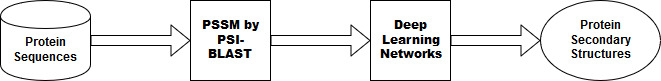
\includegraphics[width=\textwidth]{Arch.jpg}
    \caption{Flow Chart of Proposed Methodology}
    \label{fig:my_label}
\end{figure}
\subsubsection{Generation of Sequence Profiles}
\paragraph{}
The main design goal of this prediction method was to make the entire system easily ported to any workstation. This aim encompasses both the generation of sequence profiles and the actual prediction of secondary structure. Standard approaches to generating sequence profiles are cumbersome and time-consuming. The prediction accuracy of methods based on multiple sequence alignments has been found to correlate with the degree of divergence present in the aligned set of sequences. Alignments which incorporate sequences with significant yet low sequence similarity to the target protein produce more accurate predictions that those which incorporate sequences which are very closely related to the target. With suitable choices of parameters and filtering of the search data banks, PSI-BLAST greatly outperforms a standard Smith-Waterman \cite{1} (Smith \& Waterman, 1981) search in its ability to detect distant homologues of a query sequence. In addition to this, PSI-BLAST \cite{2} generates sequence profiles as part of the search process, and here we explore the idea of using these intermediate PSI-BLAST profiles as a direct input to a secondary structure prediction method rather than extracting the sequences, and producing an explicit multiple sequence alignment as a separate step.
\paragraph{}
The position specific scoring matrices generated by PSI-BLAST will be used as input to the deep leaning network. This matrix has 20 X M elements, where M is the length of the target sequence, and each element represents the log-likelihood of that particular residue substitution at that position in the template (based on a weighted average of BLOSUM62 matrix scores for the given alignment position). Depending on the coverage of the hits obtained, different parts of this profile may be based on multiple sequences or just the query sequence itself (in which case the profile elements are identical to the appropriate row or column in the BLOSUM62 matrix). PSI-BLAST uses a simple but effective scheme for weighting the contribution of locally different numbers of sequences to the resulting profiles, and here no attempt was made to further adjust for such biases. The profile matrix elements are scaled to the required 0-1 range by using the standard sigmoid function. This scaling could also have been achieved by adapting the input units directly to accept input in the given range.
\subsubsection{Deep Learning Network Architectures}
\paragraph{}
We are proposing two approaches for building the deep learning network architecture framework. The first one is \textbf{Extreme Learning Machine (ELM) with LSTM. Extreme learning machines} \cite{8,9} are feedforward neural networks for classification, regression, clustering, sparse approximation, compression and feature learning with a single layer or multiple layers of hidden nodes, where the parameters of hidden nodes (not just the weights connecting inputs to hidden nodes) need not be tuned. These hidden nodes can be randomly assigned and never updated (i.e. they are random projection but with nonlinear transforms), or can be inherited from their ancestors without being changed. In most cases, the output weights of hidden nodes are usually learned in a single step, which essentially amounts to learning a linear model. We will be using Extreme Learning Machines for the fast training of Deep Learning Networks and for the prediction of Protein Secondary Structures from a given protein sequence. In most cases, ELM is used as a single hidden layer feedforward network (SLFN) including but not limited to sigmoid networks, RBF networks, threshold networks, fuzzy inference networks, complex neural networks, wavelet networks, Fourier transform, Laplacian transform, etc. Due to its different learning algorithm implementations for regression, classification, spare coding, compression, feature learning and clustering, multi ELMs have been used to form multi hidden layer networks, deep learning or hierarchical networks. A hidden node in ELM is a computational elements, which need not be considered as classical neuron. A hidden node in ELM can be classical artificial neurons, basis functions, or a subnetwork formed by some hidden nodes. Given any non constant piece-wise continuous function as the activation function in SLFNs, if tuning the parameters of hidden nodes can make SLFNs approximate any target function f(x), then SLFNs with random hidden layer mapping h(x) can separate arbitrary disjoint regions of any shapes. \textbf{Long short-term memory} (LSTM) units are units of a recurrent neural network (RNN). An RNN composed of LSTM units is often called an LSTM network. A common LSTM unit is composed of a cell, an input gate, an output gate and a forget gate. The cell remembers values over arbitrary time intervals and the three gates regulate the flow of information into and out of the cell. LSTMs were developed to deal with the exploding and vanishing gradient problems that can be encountered when training traditional RNNs. Relative insensitivity to gap length is an advantage of LSTM over RNNs, hidden Markov models and other sequence learning methods in numerous applications. We will use LSTM to capture the long-range interactions between amino-acid residues.
\paragraph{}
The second one is \textbf{Random Multimodal deep Learning (RMDL)} ensembler which is a new ensemble, deep learning approach for classification. RMDL solves the problem of finding the best deep learning structure and architecture while simultaneously improving robustness and accuracy through ensembles of deep learning architectures. RDML can accept as input a variety data to include text, video, images, and symbolic. Random Multimodel Deep Learning (RDML) architecture for classification. RMDL includes 3 Random models, one DNN classifier at left, one Deep CNN classifier at middle, and one Deep RNN classifier at right (each unit could be LSTM or GRU). In short, RMDL trains multiple models of Deep Neural Network (DNN), Convolutional Neural Network (CNN) and Recurrent Neural Network (RNN) in parallel and combines their results to produce better result of any of those models individually. To create these models, each deep learning model has been constructed in a random fashion regarding the number of layers and nodes in their neural network structure. The resulting RDML model can be used for various domains such as text, video, images, and symbolic.
\paragraph{}
For the performance measure of our proposed method, we will evaluate two scores, namely, Q3 Accuracy and Segment Overlap (Sov) score.
\section{Conclusion and Future Work}
\paragraph{}
The Protein secondary structure prediction can be used in for the prediction of protein tertiary structure, for protein-protein interactions, and for drug discovery, depending upon the prediction efficiency. The more efficiently we predict the secondary structure, more efficiently we can predict the tertiary structures and get the functional information about those protein sequences. 
\paragraph{}
The future work is to find a set of features which will efficiently train model and will optimize the protein secondary structure prediction results.
\clearpage
\section{Time line of the project}
\begin{table}[htp]
\centering
\caption{Time line for completion of project}
\label{my-label}
\begin{tabular}{|
>{\columncolor[HTML]{EFEFEF}}l |l|l|l|l|l|l|}
\hline
\cellcolor[HTML]{CBCEFB}\textbf{Milestone} &                                      &                                &                                &                                &                                &                                    \\ \hline
Feasibility Study                          & \cellcolor[HTML]{C0C0C0}Jul-Sep 2018 &                                &                                &                                &                                &                                    \\ \hline
Objective 1                                &                                      & \cellcolor[HTML]{C0C0C0}Oct 18 &                                &                                &                                &                                    \\ \hline
Objective 2                                &                                      &                                & \cellcolor[HTML]{C0C0C0}Nov 18 &                                &                                &                                    \\ \hline
Objective 3                                &                                      &                                &                                & \cellcolor[HTML]{C0C0C0}Nov 18 - Dec 18 &                                &                                    \\ \hline
Objective 4                                &                                      &                                &                                &                                & \cellcolor[HTML]{C0C0C0}Dec 18 &                                    \\ \hline
Final Submission                           &                                      &                                &                                &                                &                                & \cellcolor[HTML]{C0C0C0}Jan 19 - May 19 \\ \hline
\end{tabular}
\end{table}
\clearpage
\addcontentsline{toc}{section}{References}
\begin{thebibliography}{}
\bibitem{1}
Smith, T.F. \& Waterman, M.S., “Identification of Common Molecular Subsequences”, Journal of Molecular Biology, Vol. 147, No. 1, Page No. 195-197, 1981.
\bibitem{2}
Altschul, S.F., madden, T.L., Schaffer, A.A., Zhang, J.H., Zhang, Z., Miller, W., \& Lipman, D.J., “Gapped BLAST and PSI-BLAST: a new generation of protein database search programs”, Nucleic Acids Research, Vol. 25, No. 17, Page No. 3389-3402, 1997.
\bibitem{8}
 Guang-Bin Huang, Qin-Yu Zhu, Chee-Kheong Siew, "Extreme learning machine: a new learning scheme of feedforward neural networks", IEEE International Joint Conference on Neural Networks, (IJCNN'2004), Vol. 2, Page No. 985-990, 2004.
 \bibitem{9}
 Guang-Bin Huang, Qin-Yu Zhu, Chee-Kheong Siew, "Extreme learning machine: theory and applications", Neurocomputing, Vol. 70, N0. 1-3, Page No. 489-501, 2006.
\bibitem{3}
David T. Jones, “Protein secondary structure prediction based on position-specific scoring matrices”, Journal of Molecular Biology, Vol. 292, No. 2, Page No. 195-202, 1999.
\bibitem{4}
Guoren Wang, Yi Zhao, Di Wang “A protein secondary structure prediction framework based on the Extreme Learning Machine”, Neurocomputing, Vol. 72, No. 1-3, Page No. 262-268, 2008.
\bibitem{5}
Amouda Venkatesan, Jeyakodi Gopal, Manimozhi Candavelou, Sowjanya Gollapalli, "Computational Approach for Protein Structure Prediction", Healthcare Informatics Research, Vol. 19, No. 2, Page No. 137-147, 2013
\bibitem{6}
Matt Spencer, Jesse Eickholt, and Jianlin Cheng, “A Deep learning Network Approach to ab initio Protein Secondary Structure Prediction”, IEEE/ACM Transactions on Computational Biology and Bioinformatics, Vol. 12, No. 1, Page No. 103-112, 2015 
\bibitem{7}
Yanbu Guo, Bingyi Wang, Weihua Li, Bei Yang, "Protein secondary structure prediction improved by recurrent neural networks integrated with 2-dimensional convolutional neural networks", Journal of Bioinformatics and Computational Biology, 2018
\end{thebibliography}

\end{document}